%----------------------------------------------------------------------------------------------------=
%-----------------------------------------------------------------------------------------------------
% Define Document Class, and include/import the multiple libraries used to create this document 
%-----------------------------------------------------------------------------------------------------
\documentclass[12pt]{article}
\usepackage{amsmath}
\usepackage[sc]{mathpazo}
\usepackage{geometry}
\usepackage{datetime}
\usepackage[myheadings]{fullpage}
\usepackage{fancyhdr}
\usepackage{lastpage}
\usepackage{graphicx, wrapfig, subcaption, setspace, booktabs}
\usepackage[T1]{fontenc}
\usepackage[font=small, labelfont=bf]{caption}
\usepackage{fourier}
\usepackage[protrusion=true, expansion=true]{microtype}
\usepackage[english]{babel}
\usepackage{sectsty}
\usepackage{url, lipsum}
\usepackage{hyperref,bookmark}
\usepackage[T1]{fontenc}
\usepackage{amssymb}
\usepackage{listings}
\usepackage{xcolor}
\usepackage{tabularx}
\usepackage{longtable}
\usepackage{setspace}
\usepackage{float}
\usepackage{bigfoot} % to allow verbatim in footnote
\usepackage[framed,numbered,autolinebreaks,useliterate]{matlab-prettifier}
\usepackage{filecontents}
\usepackage[ruled,linesnumbered]{algorithm2e}

%-----------------------------------------------------------------------------------------------------
% Define the heading for this document
%-----------------------------------------------------------------------------------------------------
% Heading style, calling fancy header library
\pagestyle{fancy}
\fancyhf{}
\setlength\headheight{15pt}
%%%% PUT YOUR NAME HERE FOR YOUR HEADING %%%%
\fancyhead[L]{Luis Fernando Enriquez-Contreras}
\fancyhead[R]{EE 105 Lab 3 Solution}
\fancyfoot[R]{Page \thepage\ of \pageref{LastPage}}

%-----------------------------------------------------------------------------------------------------
% Set coding for in LaTeX for Matlab
%-----------------------------------------------------------------------------------------------------
\lstset{
	style              = Matlab-editor,
	basicstyle         = \mlttfamily,
	escapechar         = ",
	mlshowsectionrules = true
}

% The workflow of the document begins here
\begin{document}
	%-------------------------------------------------------------------------------
	% Title
	%-------------------------------------------------------------------------------
	\begin{titlepage}
		
		\newcommand{\HRule}{\rule{\linewidth}{0.5mm}} % Defines a new command for the horizontal lines, change thickness here
		
		\center % Center everything on the page
		
		%---------------------------------------------------------
		%	HEADING SECTIONS
		%---------------------------------------------------------
		
		\textsc{\LARGE University of California, Riverside}\\[1.5cm] % Name of your university/college
		\textsc{\Large Bourns College of Engineering}\\[0.5cm] % Major heading such as course name
		\textsc{\large Department of Electrical and Computer Engineering}\\[0.5cm] % Minor heading such as course title
		
		%---------------------------------------------------------
		%	TITLE SECTION
		%---------------------------------------------------------
		
		\HRule \\[0.6cm]
		{\Large EE 105 Lab 3 Solution \\ \normalsize First-order systems in Simulink}\\[0.4cm] % Title of your document
		\HRule \\[1.0cm]
		
		%---------------------------------------------------------
		%	AUTHOR SECTION
		%---------------------------------------------------------
		
		%\begin{minipage}{0.4\textwidth}
		\begin{center} \large
			% \emph{Authors:}  
			\medskip
			%%% PUT YOUR NAME HERE %%%
			{\textsc{\textbf{Luis Fernando Enriquez-Contreras} }} 
		\end{center}
		%\end{minipage}
		
		
		%---------------------------------------------------------
		%	DATE SECTION
		%---------------------------------------------------------
		\begin{center}
			%			\selectlanguage{USenglish}
			{\large }
		\end{center}
		% Date, change the \today to a set date if you want to be precise
		
		%---------------------------------------------------------
		%	LOGO SECTION
		%---------------------------------------------------------
		%\vfill
		\newcommand*{\plogo}{
\includegraphics{Code/Fig/UC_Riverside_seal.pdf}}
		%		\newcommand*{\plogo}{
\includegraphics[width=0.25\textwidth]{UC_Riverside_seal.pdf}}
		
		\plogo\\[1cm] % Include a department/university logo - this will require the graphicx package
		
		%---------------------------------------------------------
		
		\vfill % Fill the rest of the page with whitespace
	\end{titlepage}
	
	\newpage
	
	%-------------------------------------------------------------------------------
	% Table of Contents and Figures
	%-------------------------------------------------------------------------------
	%	\doublespacing
	\tableofcontents
	\pagebreak
	\listoffigures
	%	\listoftables
	\lstlistoflistings  
	\pagebreak
	
	%-------------------------------------------------------------------------------
	% BODY
	%-------------------------------------------------------------------------------
	
	\section{Introduction}
	%%% PUT INTRODUCTION HERE %%%
	This laboratory introduces Simulink through the analysis and design of linear ordinary differential equations (ODEs). You will explore key systems concepts like transfer functions, time constants, pole locations, DC gain, and frequency response. The design process involves choosing system parameters to meet specific requirements, using transfer functions for analysis and state-space representation for simulation testing. The lab starts with fundamental concepts in first-order systems and progressively generalizes them to higher-order systems.
	
	
	\section{Pre-Lab}
		%%% Insert Figure Here as a .pdf File %%%
		\subsection{Part 1}
			\begin{figure}[H]
			\centering
			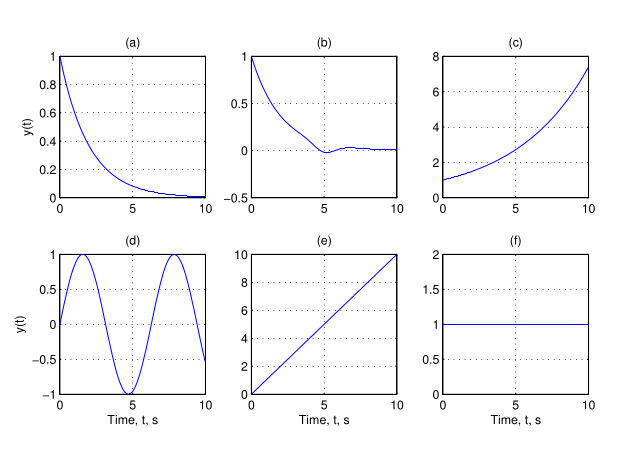
\includegraphics[width=1\linewidth]{"Code/Fig/prelab_part1.png"}
			\caption{Figures for the Prelab Part 1}
			\label{fig:prelab}
		\end{figure}
		\begin{itemize}
			\item (a) Only graphs (a), (c), and (f) from Figure \ref{fig:prelab} could correspond to a first order linear system, as none of the other graphs were exponential.
			\item (b) Graphs (b), (d), and (e) did not match the form of a decaying function.
			\item (c) \begin{itemize}
				\item (f) Parameter $a$ has the value zero, and thus never decays.
				\item (c)  has a positive value for its parameter a, thus the system is unstable
				\item (a)  has a negative value for a, thus it is stable. We can then use the initial value of that graph,
				y(0) = 1, $a$ = -.460517 therefore, $\tau$ = 2.2 seconds
			\end{itemize}
		\end{itemize}
		
		\subsection{Part 2}
		\begin{equation}
			\begin{aligned}
				\mathrm{H}(\mathrm{s})=\mathrm{Y}(\mathrm{s}) / \mathrm{U}(\mathrm{s})=\frac{1}{s R C+1} \\ 	\mathrm{H}(\mathrm{s})=\mathrm{Y}(\mathrm{s}) / \mathrm{U}(\mathrm{s})=\frac{\frac{1}{R C}}{s+\frac{1}{R C}}
			\end{aligned}
		\end{equation}
		
		\begin{equation}
			\begin{aligned}
				\frac{d x}{d t} & =\left[\frac{-1}{\mathrm{RC}}\right] x+\left[\frac{1}{\mathrm{RC}}\right] u \\
				y & =[1] x
			\end{aligned}
		\end{equation}
		\subsection{Part 3}
		\begin{equation}
			\begin{aligned}
				H(j \omega) & = Y(j \omega) / U(j \omega)=\frac{100-j \omega * 10}{100+\omega^2} \\
				\quad|H(j \omega)| & = \frac{10}{\sqrt{100+\omega^2}} \\
				\quad \angle H(j \omega) & = \arctan (-\omega / 10) \\
			\end{aligned}
		\end{equation}
		
		\begin{table}[H]
			\centering
			\caption{Magnitude and Phase for RC Circuit}
		\begin{tabular}{|c|c|c|c|c|}			
			\hline$\omega, \mathrm{rad} / \mathrm{s}$ & $|H(j \omega)|$ & $20 \log |H(j \omega)|$ & $\angle H(j \omega) \mathrm{rad}$ & $\angle H(j \omega)$ deg \\
			\hline 0.00 & 1 & 0 &  0.00 & $0^{\circ}$ \\
			\hline 0.01 & 1& 0 & -0.001 & $-0.057^{\circ}$ \\
			\hline 0.10 & 1  & 0 & -0.01 & $-0.573^{\circ}$ \\
			\hline 1.00 &  0.995  &-0.043 & -0.1 & $-5.711^{\circ}$ \\
			\hline 10.00 &  0.707 & -3.01& -0.785 & $-45^{\circ}$ \\
			\hline 100.00 & 0.1 & -20.43 & -1.471  & $-84.289^{\circ}$ \\
			\hline
		\end{tabular}
		\label{tab:rc}
	\end{table}
		\subsection{Part 4}
		\begin{figure}[H]
			\centering
			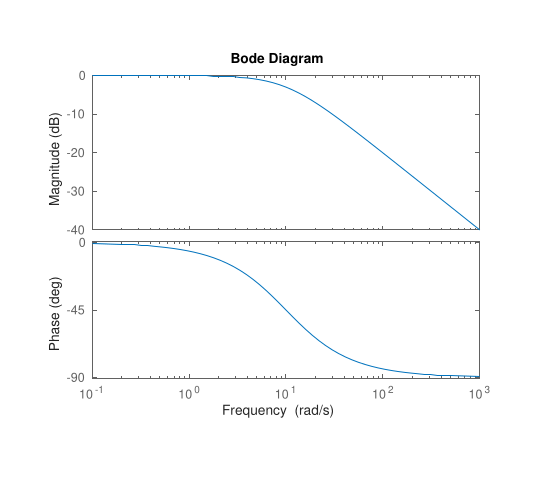
\includegraphics[width=1\linewidth]{"Code/Fig/prelab_bode.png"}
			\caption{Bode Plot for RC Circuit}
			\label{fig:bode}
		\end{figure}
		Figure \ref{fig:bode} matches the values in Table \ref{tab:rc}. 
		\newpage
	\section{Time Constant Estimation}
		%%% INSERT CODE HERE AS A .m FILE %%%
		\lstinputlisting[language=Matlab, caption = {\Large Matlab Code for Time Constant Estimation}]{"Code/time_constant_estimation.m"}	
			$\tau$  from both methods is $\approx$ 0.15.
		%%% Insert Figure Here as a .pdf File %%%
		\begin{figure}[H]
			\centering
			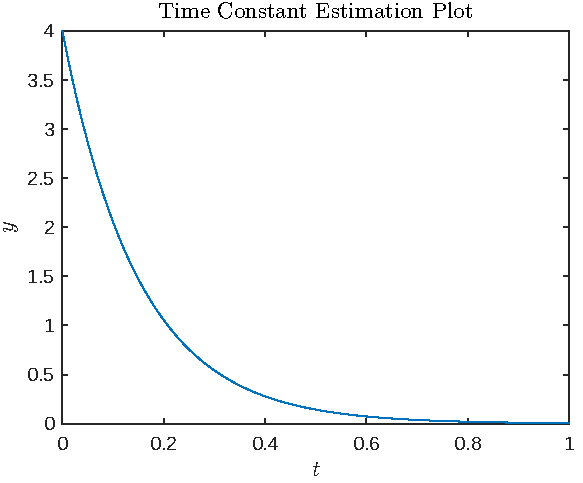
\includegraphics[width=1\linewidth]{"Code/Fig/time_constant_plot.pdf"}
			\caption{Time Constant Estimation Plot}
			\label{fig:time_constant_plot}
		\end{figure}
		% Answer questions pertaining to the section below
	  	0.37 $\times$ 4 i$\approx$ 1.5, so $t$ is $\approx$ 0.15.
	\section{Simulation with Simulink}
		\subsection{Zero Input Response}
			\begin{figure}[H]
				\centering
				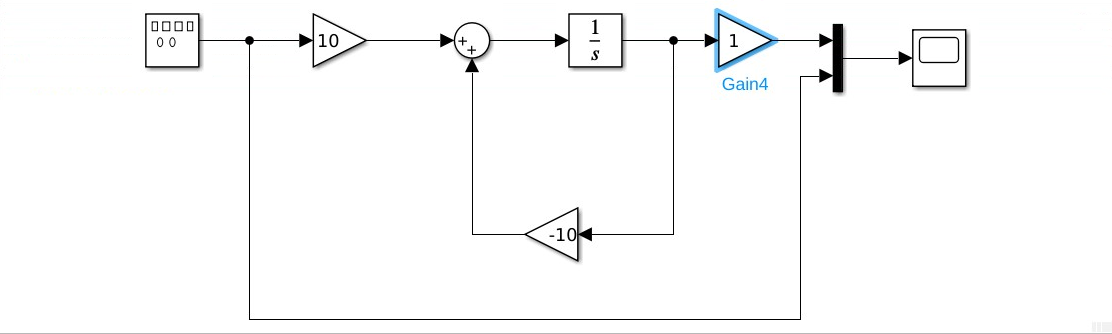
\includegraphics[width=1\linewidth]{"Code/Fig/part2_1_slx.png"} % Does not have to be a .pdf, can be another image file
				\caption{Simulink Diagram for Zero Input Response}
				\label{fig:slx_zero_input_diagram}
			\end{figure}	
			%%% Insert Figure Here as a image File %%%
			\begin{figure}[H]
				\centering
				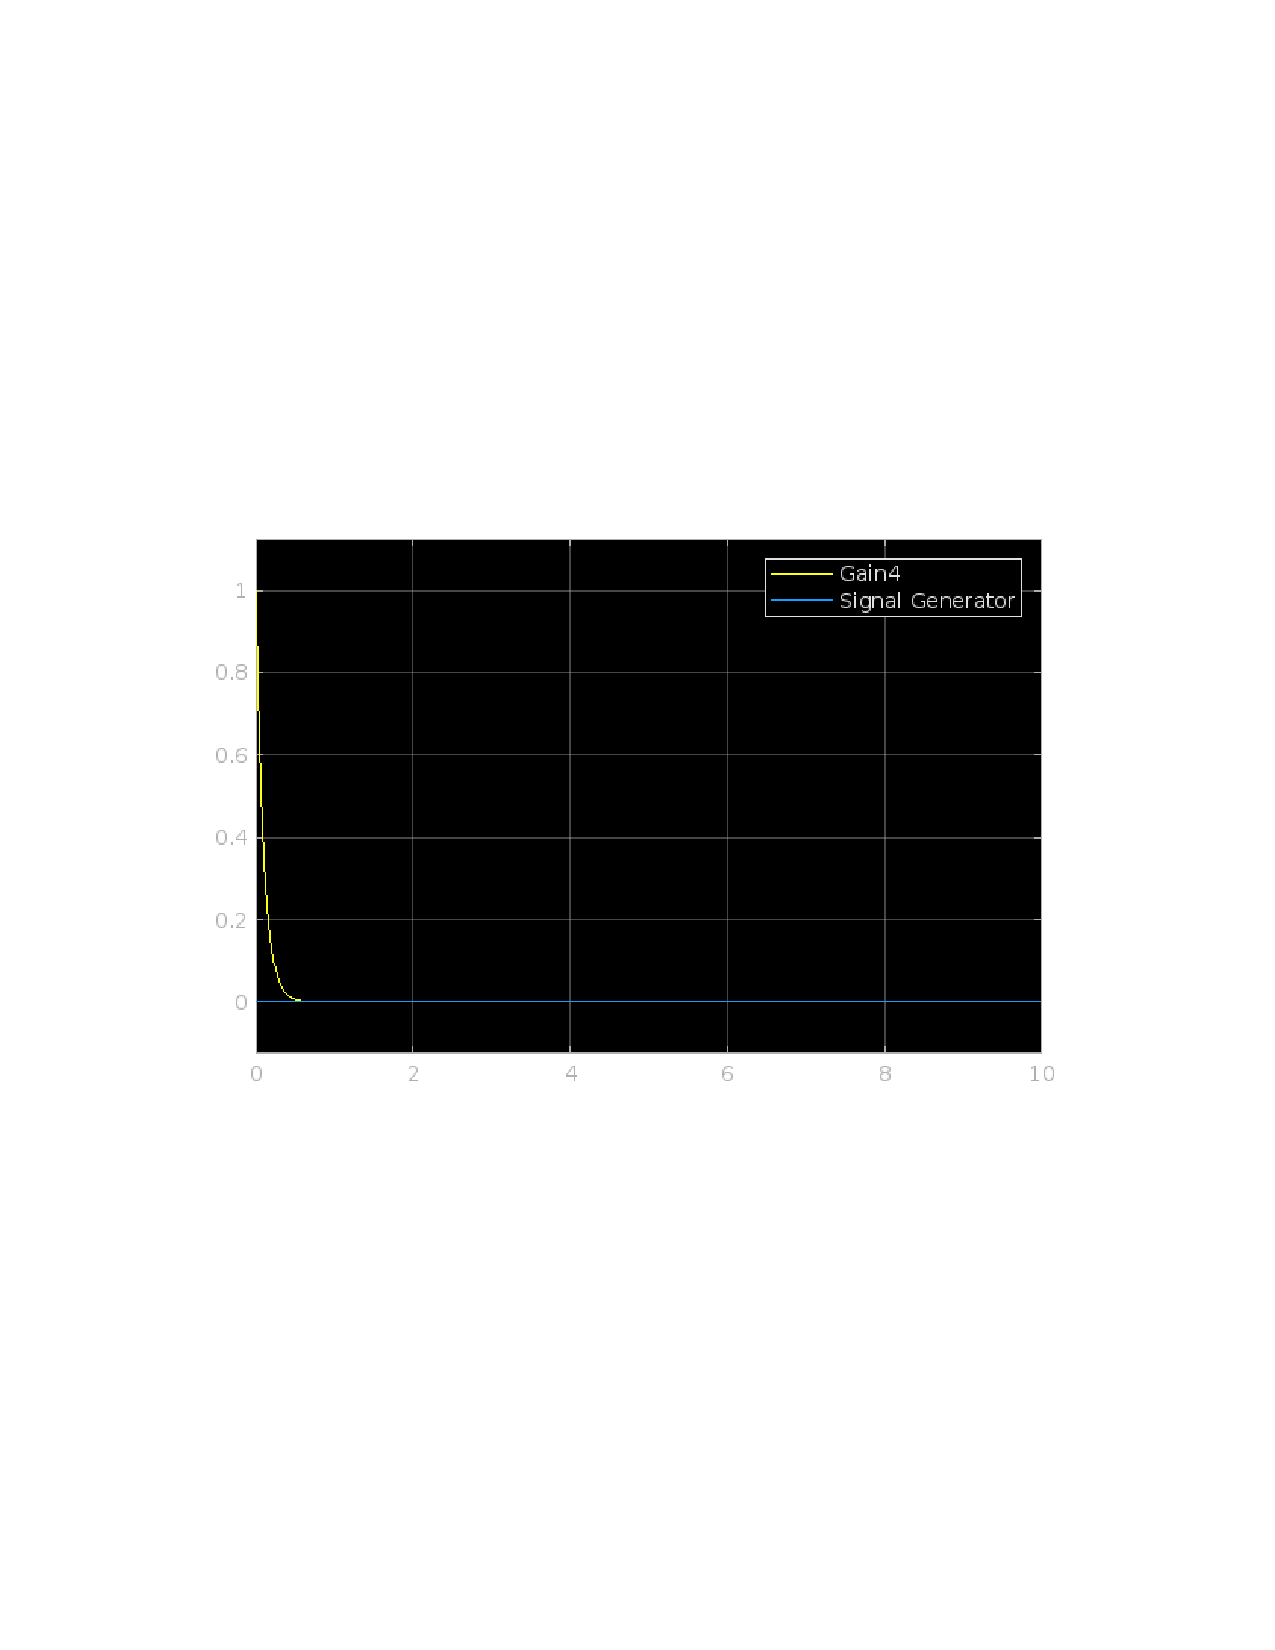
\includegraphics[width=1\linewidth]{"Code/Fig/zero_input_output.png"} 
				\caption{Oscilloscope Output of Zero Input Response}
				\label{fig:slx_zero_input_output}
			\end{figure}
			% Answer questions pertaining to the section below
			Figure \ref{fig:slx_zero_input_output} is similar to Figure \ref{fig:time_constant_plot}, and its time constant.
		\subsection{Forced Response: Step input}
			\begin{figure}[H]
				\centering
				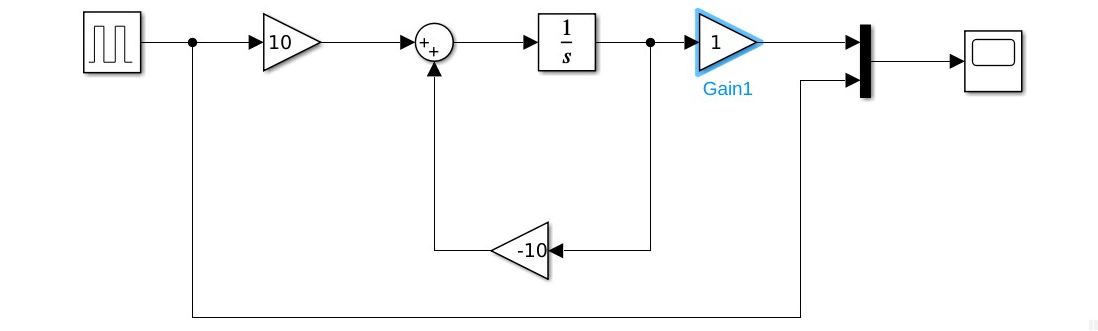
\includegraphics[width=1\linewidth]{"Code/Fig/part2_2_slx.png"} % Does not have to be a .pdf, can be another image file
				\caption{Simulink Diagram for Step Input Response}
				\label{fig:slx_step_input_diagram}
			\end{figure}	
			%%% Insert Figure Here as a image File %%%
			\begin{figure}[H]
				\centering
				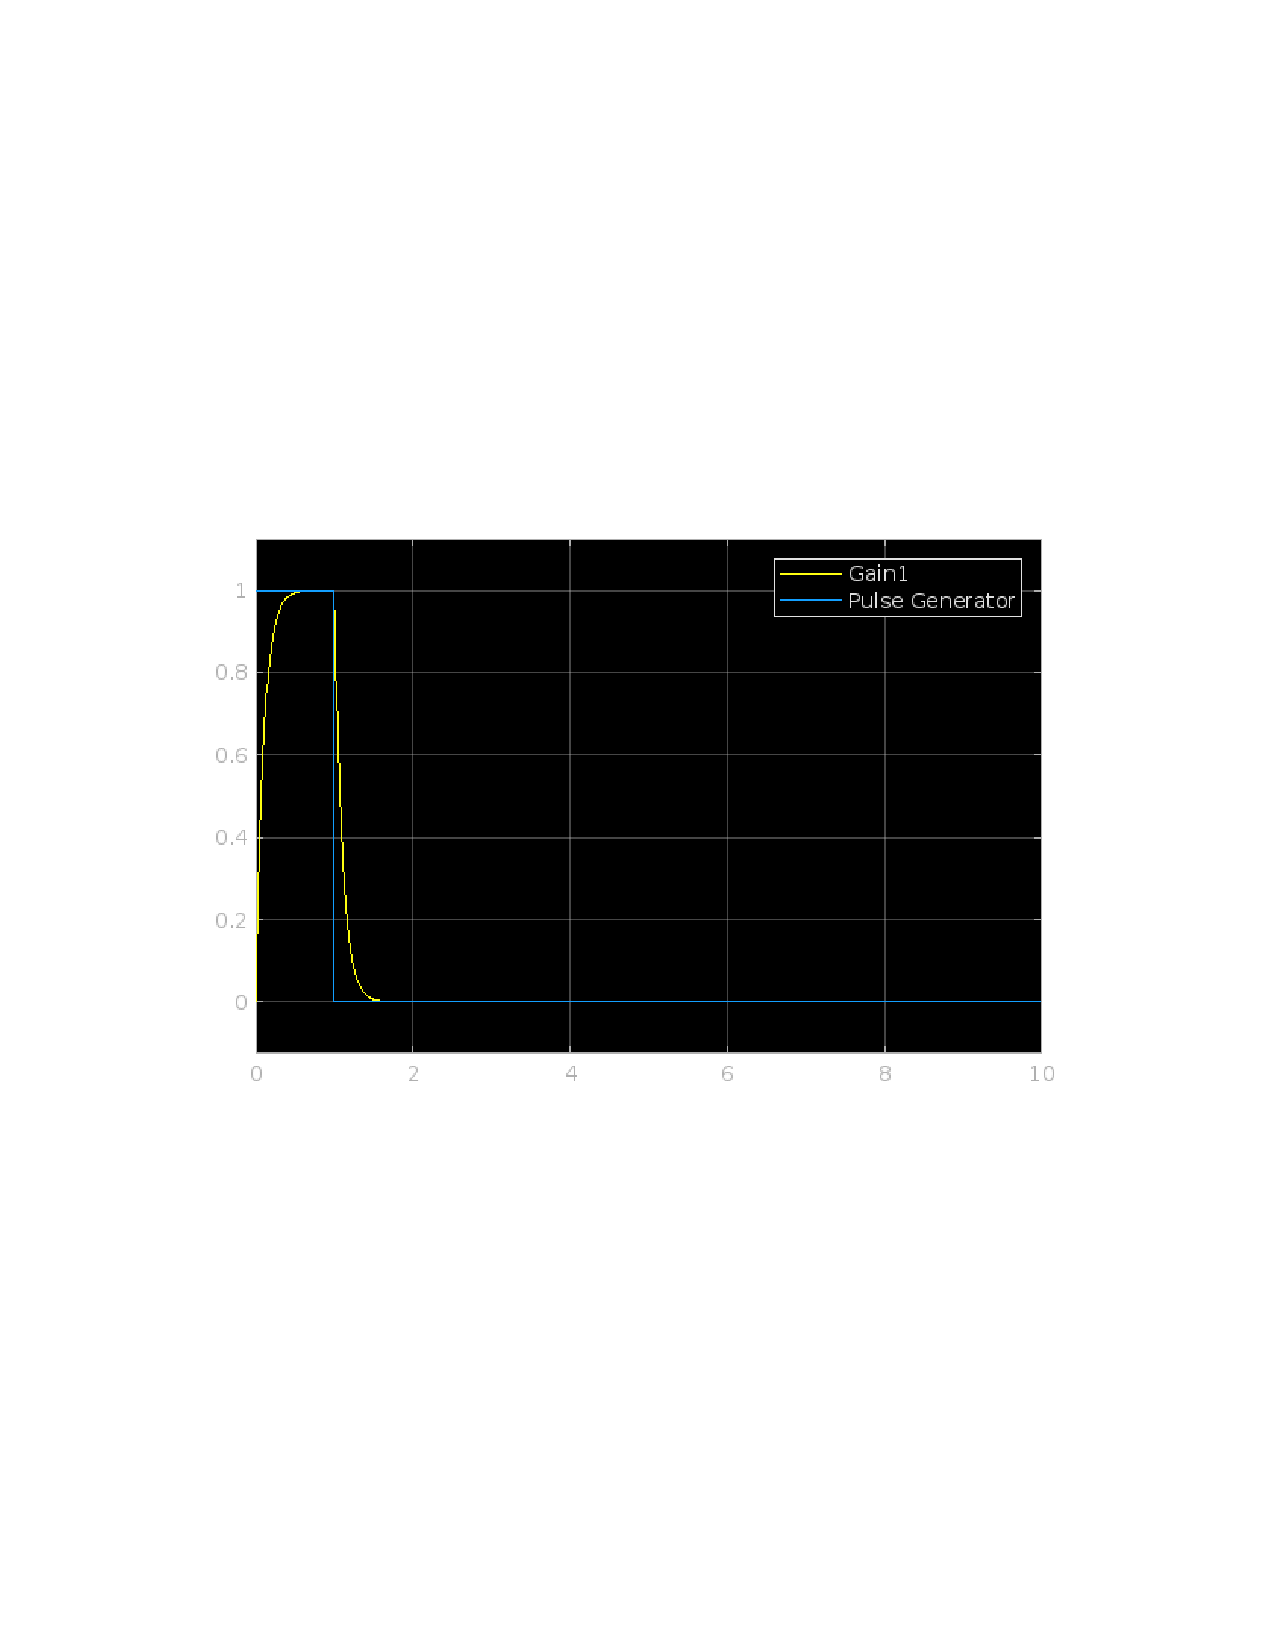
\includegraphics[width=1\linewidth]{"Code/Fig/step_input_output.png"} 
				\caption{Oscilloscope Output of Step Input Response}
				\label{fig:slx_step_input_output}
			\end{figure}
			% Answer questions pertaining to the section below
			
		\subsection{Forced Response: Sinusoidal Input}
			\begin{figure}[H]
				\centering
				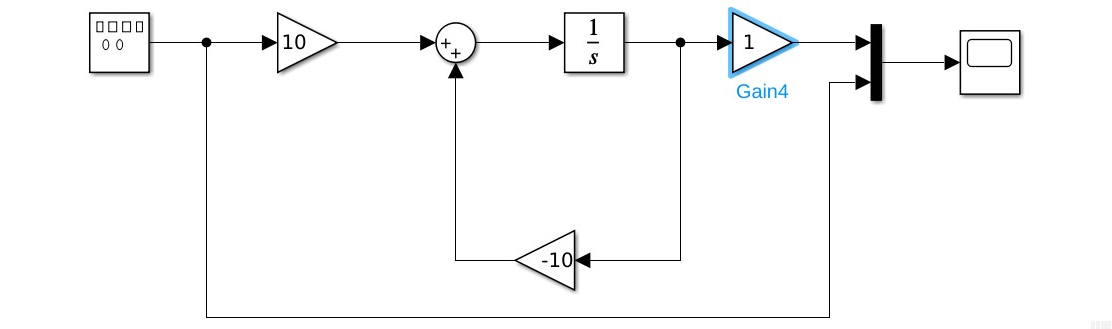
\includegraphics[width=1\linewidth]{"Code/Fig/part2_3_slx.png"} % Does not have to be a .pdf, can be another image file
				\caption{Simulink Diagram for Sinusoidal Input Response}
				\label{fig:slx_sine_input_diagram}
			\end{figure}
		
			%%% Insert Figure Here as a image File %%%		
			\begin{figure}[H]
				\centering
				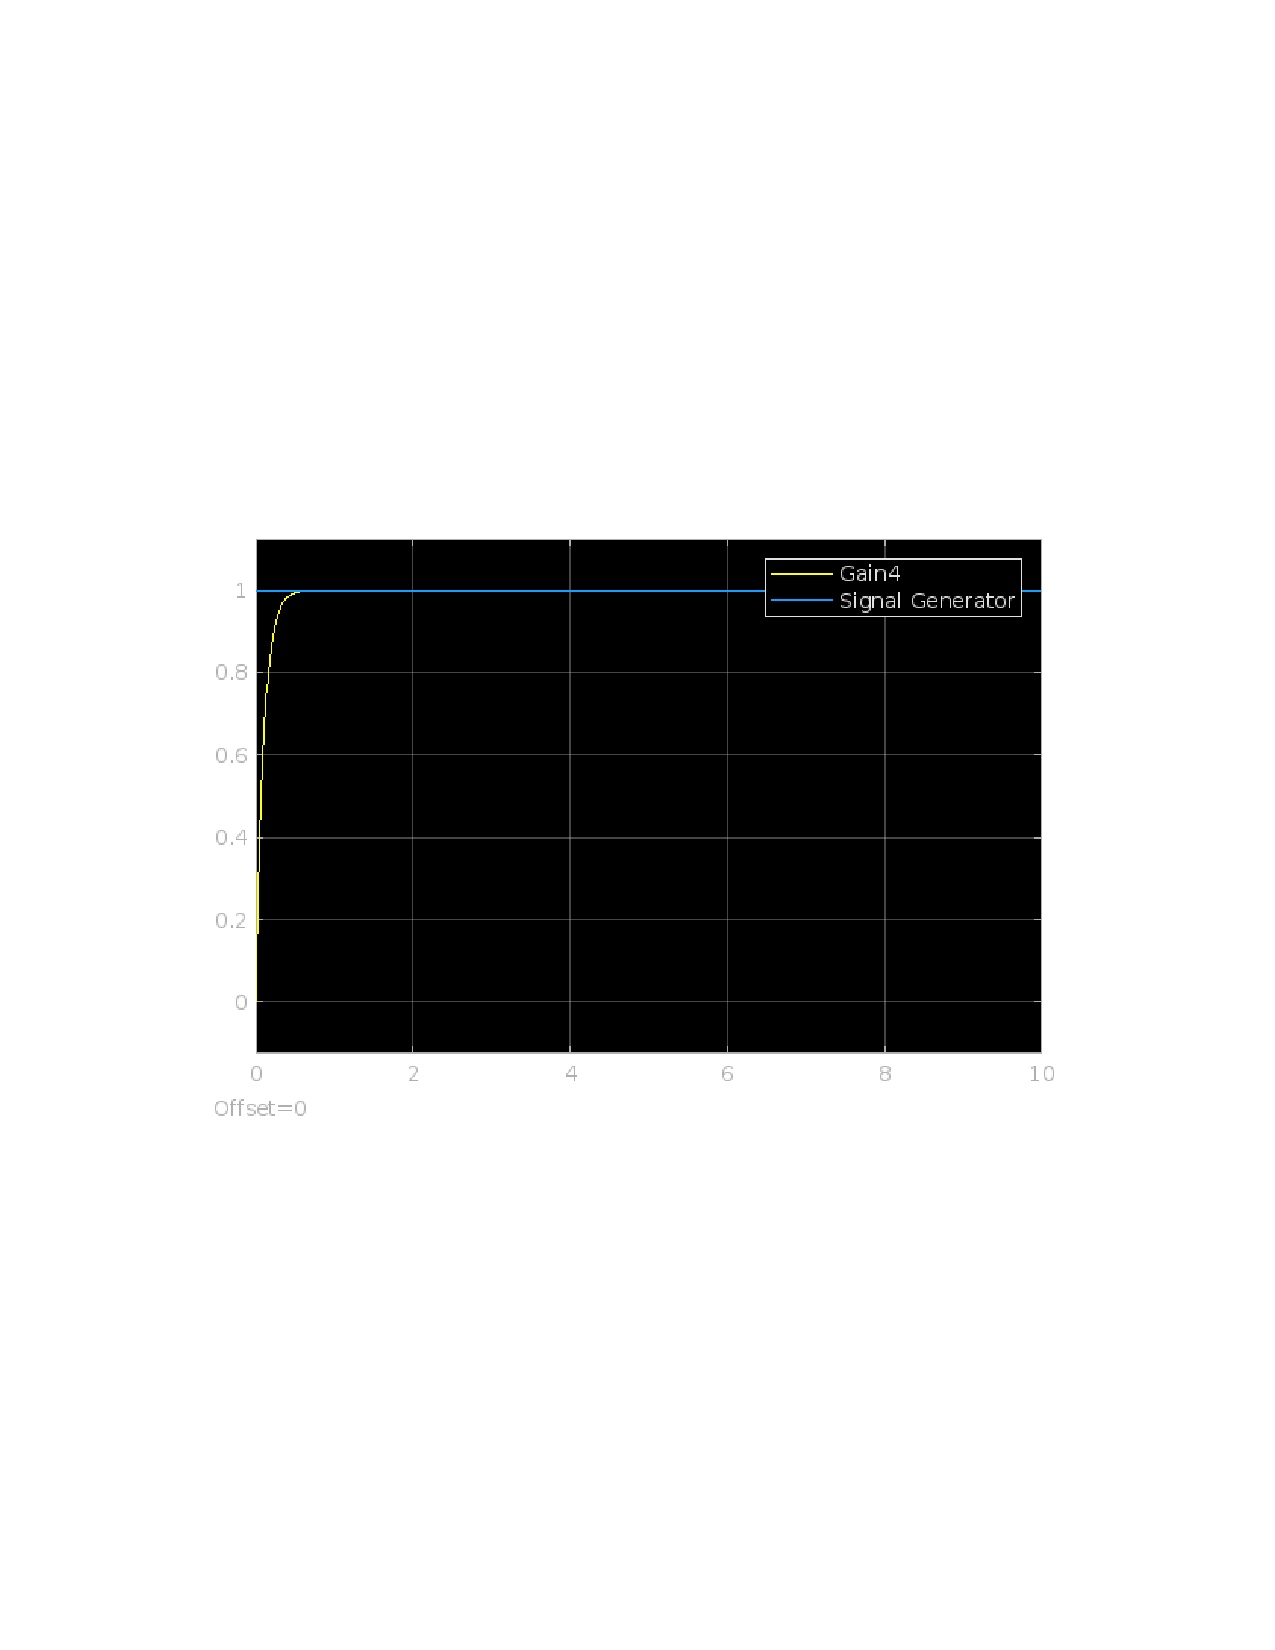
\includegraphics[width=1\linewidth]{"Code/Fig/sine_input_output_w_0.png"} 
				\caption{Oscilloscope Output of Sinusoidal Input Response $\omega$ = 0.00}
				\label{fig:slx_sine_input_output_w_0}
			\end{figure}	
			Magnitude and Phase are near identical.
			%%% Insert Figure Here as a image File %%%
			\begin{figure}[H]
				\centering
				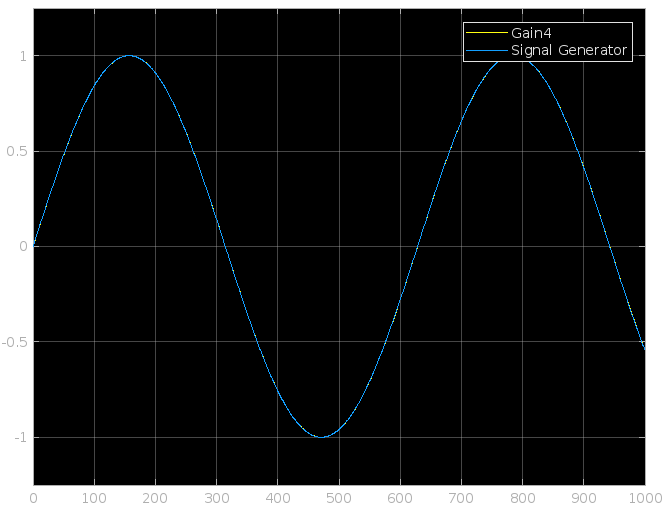
\includegraphics[width=1\linewidth]{"Code/Fig/sine_input_output_w_0_01.png"} 
				\caption{Oscilloscope Output of Sinusoidal Input Response $\omega$ = 0.01}
				\label{fig:slx_sine_input_output_w_0_01}
			\end{figure}
			Magnitude and Phase are near identical.
			%%% Insert Figure Here as a image File %%%
			\begin{figure}[H]
				\centering
				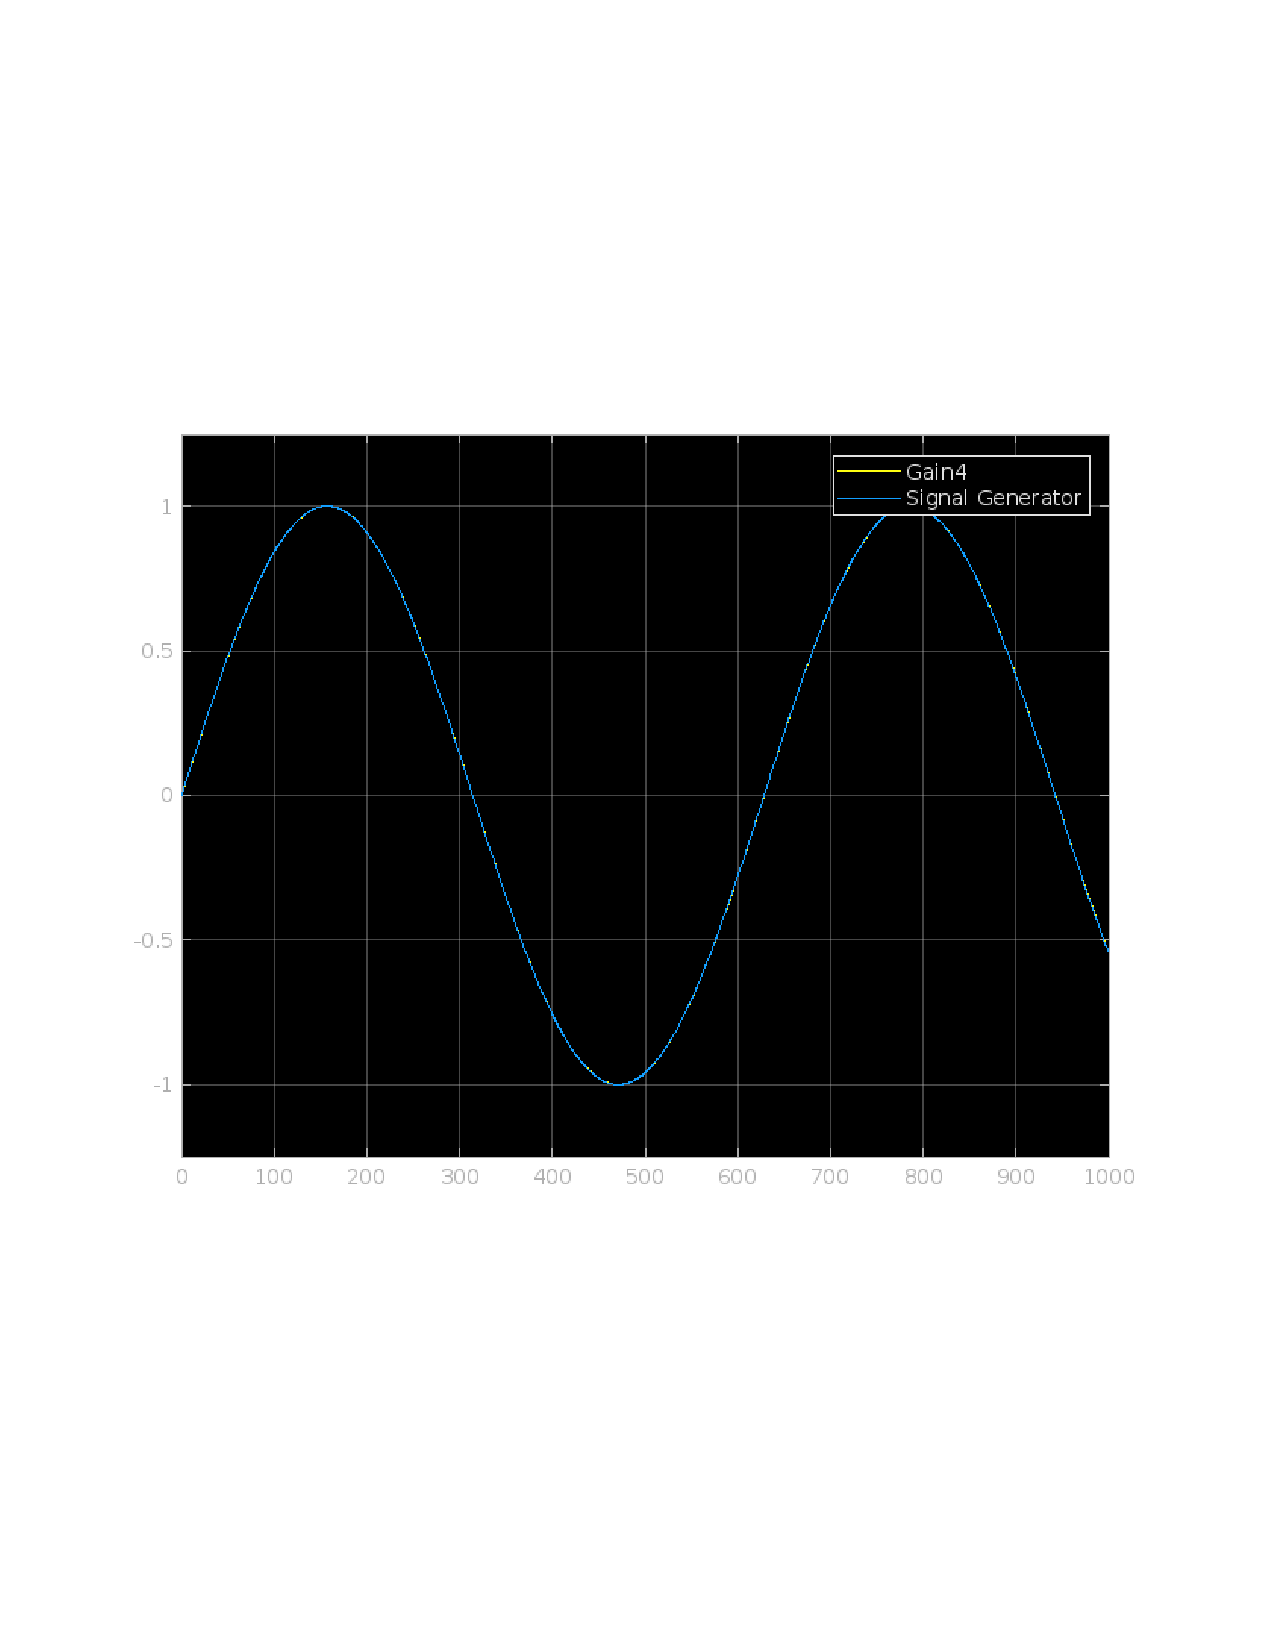
\includegraphics[width=1\linewidth]{"Code/Fig/sine_input_output_w_0_1.png"} 
				\caption{Oscilloscope Output of Sinusoidal Input Response $\omega$ = 0.10}
				\label{fig:slx_sine_input_output_w_0_10}
			\end{figure}	
			Magnitude and Phase are near identical.
			%%% Insert Figure Here as a image File %%%
			\begin{figure}[H]
				\centering
				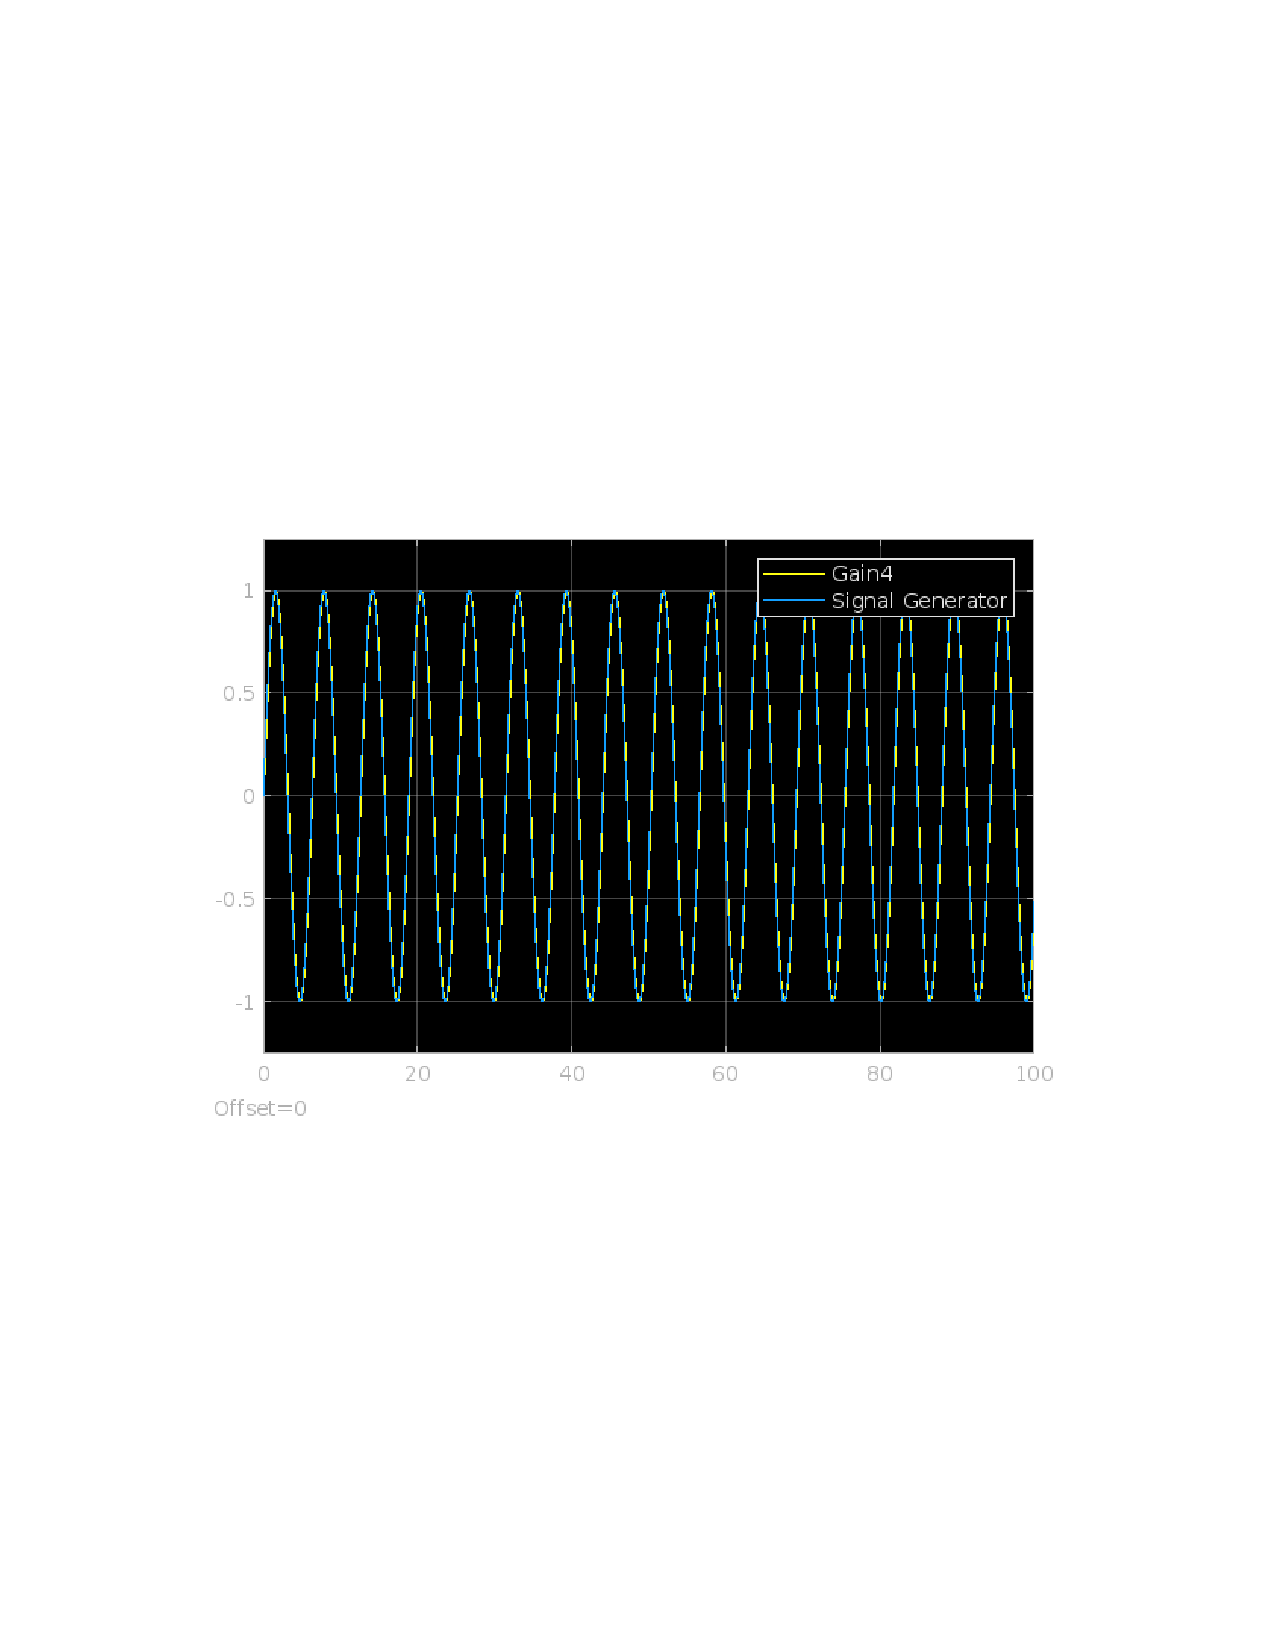
\includegraphics[width=1\linewidth]{"Code/Fig/sine_input_output_w_1.png"} 
				\caption{Oscilloscope Output of Sinusoidal Input Response $\omega$ = 1.00}
				\label{fig:slx_sine_input_output_w_1}
			\end{figure}
			Magnitude and Phase are near identical.
			%%% Insert Figure Here as a image File %%%
			\begin{figure}[H]
				\centering
				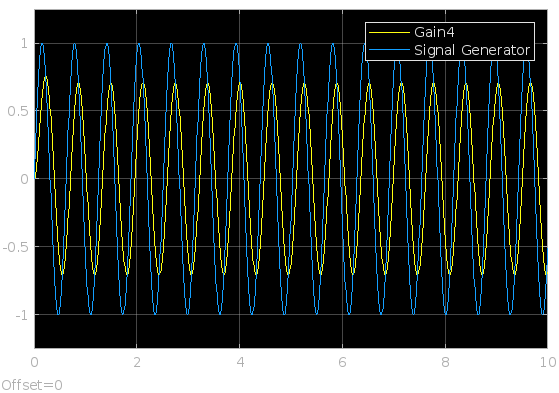
\includegraphics[width=1\linewidth]{"Code/Fig/sine_input_output_w_10.png"} 
				\caption{Oscilloscope Output of Sinusoidal Input Response $\omega$ = 10.00}
				\label{fig:slx_sine_input_output_w_10}
			\end{figure}
			\begin{figure}[H]
				\centering
				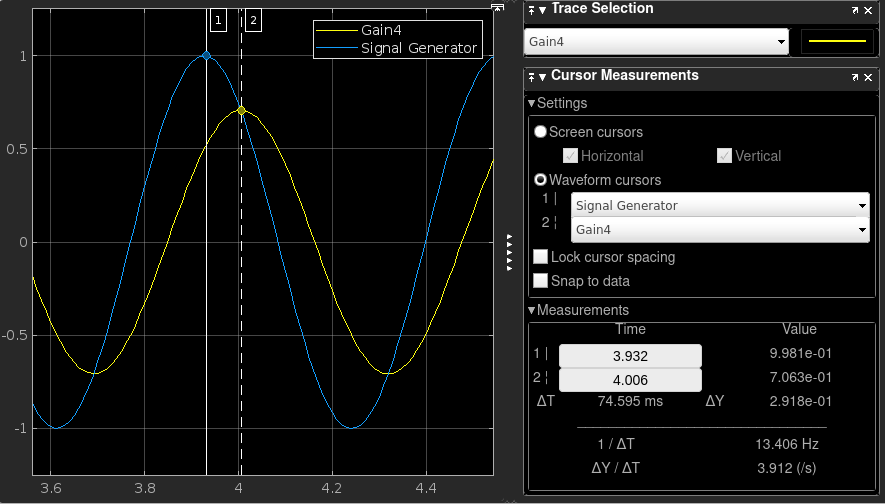
\includegraphics[width=1\linewidth]{"Code/Fig/w_10.png"} 
				\caption{Oscilloscope Magnitude and Phase Shift of Sinusoidal Input Response $\omega$ = 10.00}
				\label{fig:slx_sine_input_output_w_10_diff}
			\end{figure}
			The magnitude difference is $\approx$ .0708 and the phase shift is $\approx$ -0.746 rad.
			%%% Insert Figure Here as a image File %%%
			\begin{figure}[H]
				\centering
				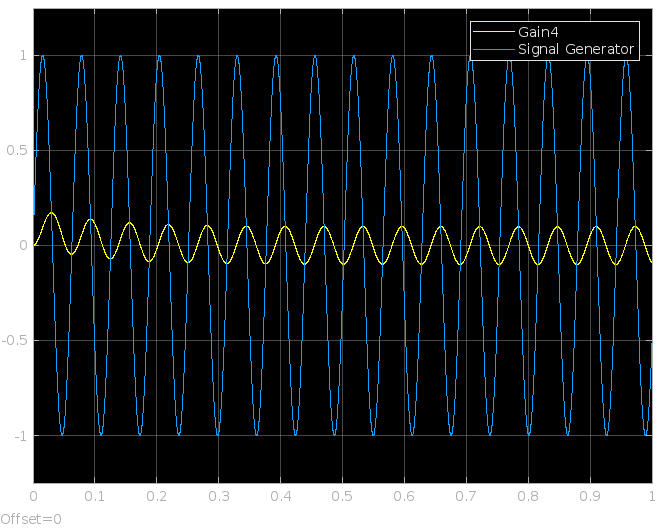
\includegraphics[width=1\linewidth]{"Code/Fig/sine_input_output_w_100.png"} 
				\caption{Oscilloscope Output of Sinusoidal Input Response $\omega$ = 100.00}
				\label{fig:slx_sine_input_output_w_100}
			\end{figure}
			\begin{figure}[H]
				\centering
				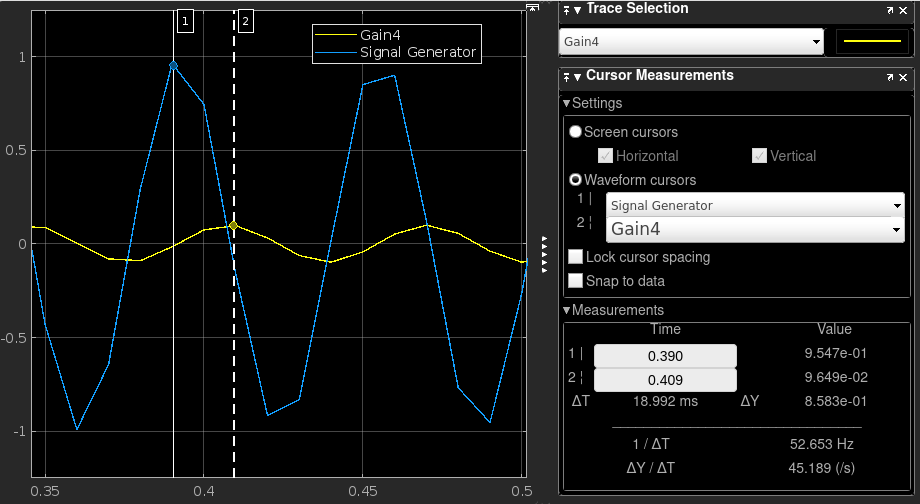
\includegraphics[width=1\linewidth]{"Code/Fig/w_100.png"} 
				\caption{Oscilloscope Magnitude and Phase Shift  of Sinusoidal Input Response $\omega$ = 100.00}
				\label{fig:slx_sine_input_output_w_100_diff}
			\end{figure}
			The magnitude difference is $\approx$ 0.102 and the phase shift is $\approx$ -1.9rad. \\
			% Answer questions pertaining to the section below
			The frequency and phase are similar to those predicted in Table \ref{tab:rc} and Figure \ref{fig:bode}. Only Figure \ref{fig:slx_sine_input_output_w_100_diff} was slight inaccurately since the plot was somewhat low resolution 
		
	\section{Conclusion}
	%%% PUT CONCLUSION HERE %%
	This lab successfully modeled a first order RC circuit using matlab and simulink to simulate the circuit.  At very low frequencies the circuits normal decay behavior, but at higher frequency the capacitor will start change the magnitude and shift the phase of an input signal. This circuit behaves as a low pass that has almost nor distortion with $\omega$ $\leq$ 1 and basically filter out sin gals where $\omega$ > 100.

\end{document}